% -*- root: ../GeometriaDiferencial.tex -*-
\chapter{Campos vectoriales y formas diferenciales: Teoremas de Frobenius y Poincaré}

\section{Campos vectoriales}
\begin{defn}[Campo\IS vectorial]
Sea $X$ un abierto de una variedad diferencial $M$. Un campo de vectores $D$ en $X$ es
una correspondencia que asigna cada punto $\vx ∈ X$ un vector $D(\vx)$ tangente a $M$ en
$\vx$.
\end{defn}

Si $\appl{f}{X}{ℝ}$ es una función diferenciable, podemos definir un campo vectorial que sea tangente a la función en cada punto.
\[\appl{D(f)}{X}{ℝ},\quad D(f)(p) := D_p(f) \]

En general, los campos son funciones de $ℝ^n$ en $\real^n$, con lo que los campos se pueden escribir $D=(f_1(x_1,...,x_n),f_2(x_1,...,x_n),...,f_n(x_1,...,x_n))$.

Lo interesante es que el espacio vectorial de los campos sobre una variedad $X$ en $ℝ^n$ tiene como base $\gen{\dpa{}{x_1},\dpa{}{x_2},...,\dpa{}{x_n}}$ con lo que los campos se pueden escriben también así:

\[D= f_1(x_1,...,x_n)\dpa{}{x_1} + f_2(x_1,...,x_n) \dpa{}{x_2} + ... + f_n(x_1,...,x_n) \dpa{}{x_n}\]

\paragraph{Operaciones con campos}

Si $\appl{f}{X}{ℝ}$ es una función diferenciable, podemos definir una nueva funcióin combinando $X$ y $f$, es decir, \textcolor{green}{(según L. Guijarro, pero no entiendo bien)}
\[\appl{D(f)}{X}{ℝ},\quad D(f)(p) := D_p(f) \]



También podemos definir el producto escalar con una función:
\[\appl{fD}{X}{ℝ},\quad (fD)(p) = f(D_p) \]

Recordamos que $\appl{D}{X⊂ℝ^n}{ℝ^n}$, con lo que la operación anterior está bien definida.

Además, nos interesa definir la suma de campos.

Si $D,D'$ son 2 campos, definimos: $(D+D')(x) := D(x) + D'(x)$

\paragraph{Ejemplos}

Sea $\appl{D_1}{ℝ^2}{ℝ^2}$ definido $ D_1=2x\dpa{}{x} + (y-1)\dpa{}{y} = (2x,y-1)$.

Sea $\appl{f}{ℝ^2}{ℝ}$, con $f(x,y) = 3xy$

Sea $\appl{D_2}{ℝ^2}{ℝ^2}$ definido $ D_2=x\dpa{}{x} + y\dpa{}{y} = (y,x)$.


$D_1(3,4) = (6,3)$

$(fD_1)(3,4) = f(6,3) = 3·6·3 = 54$

¿¿$D_1(f)(3,4) = D_1(3,4)f = (6,3)f$??

$(D_1 + D_2)(3,4) = D_1(3,4) + D_2(3,4) = (2·3 + 4, 4-1 + 3)$

\section{Curvas integrales}



Si tenemos una aplicación $\appl{F}{X}{Y}$, entonces la definición de la diferencial en un punto \[ (DF)_x = \appl{F_{*, x}}{\tgs_x }{\tgs_{F(x)} Y} \] es la misma para abiertos de $ℝ^n$ que para variedades diferenciales en $ℝ^n$.

¿Podemos \textit{llevar} el campo definido en $X$ a $Y$?

Si $F$ es inyectiva y $D$ es un campo en $X$, entonces sí existe un campo $F_*(D)$ definido no en $Y$ sino en $F(X) ⊂ Y$.

Vamos a ver varios resultados en esto.

\begin{defn}[Curva\IS integral de un campo] Sea $\appl{γ}{I}{X}$ una curva donde $I = [-a, a]$ es un intervalo simétrico alrededor del origen, y $D$ un campo en $X$. Decimos que γ es una curva integral de $D$ por el punto $x_0$ si se cumple que $γ(0) = x_0$.

Además $γ_*\left(\dpa{}{t}\right) = \restr{D}{γ(I)}$ donde $\dpa{}{t}$ es un campo  de vectores que a cada punto de la curva le asigna su vector tangente, es decir, $\dpa{}{t}γ(p) = D_p$
\end{defn}

Supongamos por ejemplo que $D = \sum a_i(x_1, \dotsc, x_n) \dpa{}{x_i}$. Entonces, dada $γ(t) = (x_1(t), \dotsc, x_n(t))$, tendríamos que \[ γ_*\left(\dpa{}{t}\right) = \sum x_i'(t) \dpa{}{x_i}\] ya que recordemos que aplicar la función es sólo permutar los símbolos: \[ γ_* \left(\dpa{}{t}\right) f = \dpa{}{t} (f○γ) \]

Al igualar $D$ con la composición esa tendríamos que, para $i = 1, \dotsc, n$, \[ x_i'(t) = a_i(x_1(t), \dotsc, x_n(t))\] Todo eso junto es un sistema de ecuaciones diferenciales ordinarias autónomo. Es decir, que el campo da lugar a un sistema de ecuaciones locales en el que aplicar los teoremas del curso de Ecuaciones diferenciales ordinarias, en los que este sistema tiene solución siempre que $D$ sea continuo.

El nombre de curva integral viene de que como $D(γ(t)) = γ'(t)$, si integramos el campo a lo largo de la curva obtenemos:

\[
\int_γ D(x) dx = \int_{-a}^a <D(γ(x)),γ'(x)> dx = \int_{-a}^a <γ'(t),γ'(t)> dx = \int_{-a}^a dx = a-(-a) = 2a = cte
\]

\paragraph{Más coceptos} Hay una definición y un teorema útiles en geometría. Vamos a verlos.

\begin{defn}[Caja] Dado $x_0$ un punto y $D$ un campo en $X$, se dice que una caja para $D$ en $x_0$ es una tripleta formada por un entorno abierto $U_0$ de $x_0$, un real $a > 0$ (o infinito) y una función $Φ$ que cumplen ciertas condiciones.

$Φ$ debe ser una función $\appl{Φ}{U_0 × (-a, a)}{X}$ diferenciable ($C^∞$). Además $∀x∈U_0$ fijo se obtiene una función $γ_x ≝ \appl{Φ(x, t)}{(-a, a)}{X}$ que define una curva integral en $X$. Dicho de otra forma, la función $Φ_0$ ``pega'' todas las curvas.

La última condición es que, $∀t ∈ (-a, a)$ fijo podemos definir una función $\appl{τ_t}{U_0}{X}$ que por definición es simplemente $τ_t ≝ Φ(x,t)$ y que cumple el ser un difeomorfismo de $U_0$ con su imagen.
\end{defn}

\begin{theorem} Para todo $D$ y $x_0 ∈ X$, existe una caja y además es única.

Además, si $t_1, t_2, t_1 + t_2 ∈ (-a, a)$, entonces $τ_{t_1+t_2} = τ_{t_1} ○ τ_{t_2} = τ_{t_2} ○ τ_{t_1}$.
\end{theorem}

Ese último enunciado del teorema nos da una especie de propiedad de grupo para τ. De hecho, a τ se le llama el \concept[Flujo\IS de un campo]{flujo de un campo}.

Por ejemplo, si vemos el campo de velocidades de un fluido estacionario, en el que la velocidad sólo depende del punto $x$ del fluido, la función $τ_t(x)$ nos da una progresión del líquido, cómo se mueven las partículas a lo largo del tiempo por la curva que pasa por $x$.

Geométricamente, un campo lo que hace es definir un flujo cuando se integra: para cada $t$, se obtiene una función que va de cada punto en el punto imagen por el flujo, y ese movimiento determina las curvas solución y está determinado por ellas, por supuesto.

En este caso, se dice que el campo es el generador infinitesimal del flujo y el flujo se dice que es el flujo del campo flujo flujo flujo.

Hay dos teoremas importantes sobre los campos.

\begin{theorem}[Enderezamiento\IS de campos] Sea $D$ un campo en $X$ y $x_0$ un punto en $X$ donde el campo no se anula ($D_{x_0} ≠ 0$). Entonces existe un sistema $y_1, \dotsc, y_n$ de coordenadas locales en un entorno de $x_0$ en el cual $D = \dpa{}{y_1}$. \label{thmEnderezamientoCampos}
\end{theorem}

Este teorema lo que está diciendo es que se puede cambiar de carta de forma que en la nueva carta el campo se escribe de una manera más sencilla de manejar. Es necesario que el campo no sea nulo, porque si no la derivada esa se anularía.

Esto es importante porque en Geometría Diferencial a veces los problemas se resuelven de manera intrínseca, sin usar coordenadas locales. Pero cuando hagamos los cálculos en coordenadas locales, elegiremos un sistema mejor adaptado al problema para hacer el cálculo como si fuera en abiertos de $ℝ^n$. Lo que dice el teorema es que nos conviene usar las coordenadas locales esas para tener una expresión lo más simple posible.

Antes de llevar a cabo la demostración, hay una definición que debemos tener clara:
\begin{defn}[Integral\IS primera] Se llaman \textbf{integrales primeras} de un campo D en un abierto U a funciones $\appl{f}{U}{\real}$ tales que $D(f)=0$ en todo punto de U.
\end{defn}

\begin{proof}
\begin{enumerate}
\item Las funciones que buscamos verifican, suponiendo el teorema demostrado,
\[D(y_1)=1, \ D(y_j)=0 \ j=2,\cdots n\]
\item La demostración comienza por considerar la curva solución por $p$ y una hipersuperficie $H$ pasando por $p$ cuyo hiperplano tangente no contenta al vector $D_p$. Por ejemplo, supongamos $a_1(p)\neq 0$ y tomamos como $H$ la hipersuperficie $x_1=0$

\item Las curvas solución por puntos de $H$ próximos a $p$ tendrán vector tangente no contenido en el hiperplano tangente a $H$ en el punto. La unión de todas esas curvas define $V$.

\item Para definir las coordenadas $y_j, \ j=2, \cdots, n$, consideramos la función $\appl{F}{V}{H}$ que a cada punto $p$ le asocia el punto de corte de la curva solución por $p$ con $H$. Sean $z_j, \ j=1, \cdots, n$ funciones coordenadas en $H\cap V$. Definimos $y_j=z_j\circ F$

\item
Las funciones $y_j$ son integrales primeras de $D$ en $V$, ya que, por construcción, las funciones $y_j$ son constantes sobre las curvas integrales del campo $D$. Por definición de curva integral
\[D(y_j)=\frac{d}{dt}(y_j \circ γ)\]
y, por tanto, vale 0

\item Falta definir la función $y_1$, usando la función que define $H$, y demostrar que $(y_1,...y_n)$ es un sistema de coordenadas en el entorno de $p$

\end{enumerate}
\end{proof}

\begin{example}
Sea $α(t) = (−t, 2 − t^2 , 2)$, y sea $D=-\dpa{}{x} -2xz \dpa{}{y}$. ¿Es $α$ una curva integral de $D$?

Para comprobarlo, calculamos $α'(t) = (-1,-2t,0)$, que tratado como campo, tendríamos $α'(t) = -1 · \dpa{}{x} + (-2t) · \dpa{}{y} + 0 \dpa{}{z} = D$, con lo que sí es una curva integral de $D$, en este caso, $∀t∈ℝ$.

\end{example}

\subsubsection{Ejemplos}
\begin{example}
Supongamos la recta real $ℝ$ con coordenada $x$, y una partícula sometida a un potencial $U(x)$. Es decir, que la fuerza sobre la partícula es $F = -U'(x)$. Sabemos que $F = ma$, luego \[ -U'(x) = F = m a = m \od[2]{x(t)}{t} = \od{p}{t} \] donde $p = m \od{x}{t} = mv$ es el momento lineal.

Vamos a hacer el cálculo en un plano $xp$, donde $x$ es la coordenada y $p$ es el momento. En estas coordenadas, $\od{x}{t} = \frac{p}{m}$. Es decir, que con este truco hemos pasado a un sistema de ecuaciones de primer orden.

Esto se puede hacer como un campo \[ D = \frac{p}{m}\pd{}{x} - U'(x) \pd{}{p} \] en el plano. Busquemos las integrales primeras del campo: funciones $H$ tales que $D(H) = 0$. Sabemos que las integrales primeras existen localmente en entornos de puntos en los que el campo no se anule.

Para encontrarla, tenemos que resolver la ecuación en derivadas parciales \[ \frac{p}{m} \pd{H}{x} - U'(x) \pd{H}{p} = 0 \]

Para resolver eso escribimos \[ \pd{H}{x} = U'(x) \qquad \pd{H}{p} = \frac{p}{m}\]

De la primera ecuación sacamos que $H(x,p) = U(x) + C(p)$. Derivando esto con respecto a $p$, tenemos que $\pd{H}{p} = C'(p) = \frac{p}{m}$, luego $C(p) = \frac{p^2}{2m}$, de tal forma que \[ H = U(x) + \frac{p^2}{2m} \]

Esta es la ecuación de la energía total del sistema o mecánica, donde $\frac{p^2}{2m}$ es la energía cinética. La energía mecánica se conserva así que eso de ahí es cosntante (y su derivada es cero).

Ahora bien, ¿qué haríamos para resolver el movimiento de la partícula? ¿Qué habría que hacer para continuar? ¿Cómo usamos el hecho de que la energía se mantiene constante?

Queremos conocer no ya la curva en el plano de fases $xp$, sino también su proyección en el eje $x$ en función del tiempo. Lo que hacemos es sustituir en la ecuación de antes $p$ por $m\od{x}{t}$, luego \[ H = U(x) + \frac{1}{2m}\left(m\od{x}{t}\right)^2 = E_0 \] donde $E_0$ es constante. Es decir, hemos pasado una ecuación de primer orden separable, que se reduce a una integral, y despejando y haciendo cosas e integrando se sale.
\end{example}

\begin{example}
Consideramos un punto $(a,b) ∈ ℝ^2$, y consideramos para cada punto $(a,b)$ la parábola $y = x^2 + (b-a^2)$, que se puede parametrizar por $γ(t) = (t, t^2 + (b-a^2))$. ¿Cómo calculamos el campo cuyas curvas solución son esas? Tenemos que derivar. Es claro que el campo será \[ D_{(x,y)} = (1,2t) \] Resolviendo el sistema $D = \pd{}{x} + 2x \pd{}{y}$ nos queda que $x(t) = t +c_1$ y que $y(t) = t^2 + 2c_1 t + c_2$, es decir, las mismas curvas de las familias de antes con $a = c_1$ y $b =c_2$. El flujo está dado por \[ τ_t(x,y) = (t, t^2 + (y-x^2))\]

Vamos a buscar también enderezar el campo. Consideramos \[ D(H) = 0 = \pd{H}{x} + 2x \pd{H}{y} \] y haciendo lo mismo de antes la solución es $H(x,y) = -x^2 + y$, que está diciendo que las curvas solución están contenidas en parábolas, cosa que ya sabíamos desde el principio.

El resto del ejemplo es demostrar que el determinante de la mariz jacobiana es no nulo en todo punto y entonces las coordenadas locales que enderazan el campo son coordenadas globales en este caso, porque en todo punto la matriz jacobiana tiene detemrinante no nulo y se comprueba de hecho que es una carta loca, lse calcula la inversa, y luego hay un segundo ejemplo que no da tiempoa mirar hoy que es en una sola variable y que nosequé.

\end{example}

\begin{example}
El otro ejemplo es el campo dado por \[ D = x^2 \pd{}{x} \] al que le corresponde la ecuación $\od{x}{t} = x^2$, luego $t = \frac{-1}{x} + C$. Despejando, \[ x = \frac{-1}{t-C} \]

Así, cuando $t = 0$, la posición en el instante inicial $x_0 = \frac{1}{C}$ y sustituyendo de vuelta tenemos que \[ x = \frac{x_0}{1-tx_0} \]

El flujo del campo es por lo tanto \[ τ_t(x) = \frac{x}{1-xt} \], que nos da para cada punto $x$ nos va a dar la trayectoria en función del tiempo. Es curioso ver que el flujo no es global porque cuando $t = \frac{1}{x}$ se hace infinito.

Esto quiere decir que hay una cierta limitación si queremos definir el flujo en todo $t$. Es una justificación de la hipótesis que vamos a enunciar ahora, o que ya enunciamos en su momento. No sé.
\end{example}

\begin{defn}[Soporte] Dado un abierto $U ⊂ ℝ^n$ y un campo $D$ en $U$. El soporte del campo se define como \[ \mop{sop}(D) ≝ \adh{\set { p ∈ U \tq D_p ≠ 0}} \] \label{defSoporte} \end{defn}

\begin{theorem} Si $\mop{sop}(D)$ es compacto y está contenido en $D$, entonces el flujo $τ_t$ está definido para todo $t∈ℝ$.
\end{theorem}

\begin{proof}
En la hoja está la idea.
\end{proof}

\section{Corchete de Lie}

Dados dos campos \[ D = \sum a_i \pd{}{x_i} \qquad \quad D' = \sum b_j \pd{}{x_j} \] y una función $f$, podemos considerar el siguiente cálculo: \[ D(D'(f)) = D\left(\sum b_j \dpa{f}{x_j} \right) = \sum_{i,j} a_i \pd{b_j}{x_i} \pd{f}{x_j} + \sum_{i,j} a_i b_j \mder{f}{2}{x_1}{}{x_j}{} \]

Así, queda claro que $D(D')$ no es un campo. Ahora bien, hay una cierta simetría que nos permite escribir:

\[ [D, D'] ≝ D○D' - D'○D = \sum_j\left(\sum_i a_i \dpa{b_j}{x_i} - b_i \dpa{a_j}{x_i}\right) \dpa{}{x_j}\]

Esto simplifica mucho las cosas ya que tiene propiedades interesantes:
\newpage
Veamos algunas de estas propiedades
\begin{enumerate}
\item $[D, D'] = - [D', D]$.
\item Bilinealidad; $[aD + bD', D''] = a[D, D''] + b[D', D'']$.
\item \concept{Identidad\IS de Jacobi}: la suma de permutación cíclica es cero: $[[D, D'], D''] + [[D',D''], D] + [[D'',D], D'] = 0$.
\item $[fD, gD'] = fg[D, D'] + fD(g)D' - gD'(f) D$
\item $[[D, D'], D''] = [DD' - D'D, D''] = DD'D'' -D''DD' - D'DD'' + D''D'D$.
\item $[fD, yD'] h = fD(gD'(h)) - gD'(fD(h))$
\end{enumerate}

Ahora bien, ¿para qué sirve esto? Vamos a verlo empezando con subvariedades.

La clave está en el siguiente link: \href{https://jadsuafu.wordpress.com/2012/09/27/calculos-tipicos-en-variedades-diferenciables-corchete-de-lie-derivada-de-lie-y-diferencial-exterior/}{Corchete de Lie}
\section{Subvariedades}

El teorema de la función inversa nos permite obtener una forma canónica local para cualquier aplicación diferenciable con diferencial de rango constante

\begin{theorem}[Teorema del rango constante]
Sea $U \subset \real^n$ un abierto. Si $\appl{F}{U}{\real^m}$ es una aplicación diferenciable tal que su diferencia $F_*$ tiene rango constante $k$ en $U(k \leq m)$, entonces para cada punto $p\in U$ hay cartas $(U, \phi)$ y $(V, \psi)$ definidas en un entorno de $F(p)$ tales que $\psi F \phi^{-1}$ es la restricción a $U$ de la proyección lineal de rango $k$
\[\real^n \to \real^m\]
\[(x_1,...,x_k,...,x_n) \to (x_1,...x_k,0,...,0)\]
\end{theorem}

Esto va en la misma línea que el teorema de enderezamiento de campos (\ref{thmEnderezamientoCampos}): nos permite cambiar las coordenadas para llegar a un sistema más fácil de manejar.

\subsection{Inmersión}
\begin{defn}[Inmersión] Sean $M$ y $N$ variedades diferenciables. Se dice que una función diferenciable $\appl{F}{M}{N}$ es una \textbf{inmersión} en $p$ si la diferencial $\appl{F_{*p}}{\tgs_pM}{\tgs_{F(p)}N}$ entre los espacios tangentes es inyectiva. Si $F$ es una inmersión para todo punto $p\in M$ decimos que es una \textbf{inmersión}

Si los abiertos en la variedad $M$ son exactamente anteimágenes por $F$ de los abiertos en $N$, decimos que la inmersión es \concept{compatible con la topología} (en inglés, embedding).

Un subconjunto $M \subset N$ de una variedad diferenciable $N$ es una subvariedad si $M$ admite una estructura de variedad diferenciable tal que la función $\appl{i}{M}{N}$ es una inmersión. si además la inmersión es compatible con la topología decimos que la subvariedad es \concept{regular}
\end{defn}

\begin{example}

\begin{wrapfigure}{r}{0.4\textwidth}
\centering
\inputtikz{III_Pez}
\caption{Un pez. Glugluglu.}
\label{figPez}
\end{wrapfigure}

Cuidado porque lo que tiene que ser inyectivo es la diferencial, no la función. Por ejemplo, si consideramos la curva de ecuación $y^2 - x^2 + x^3 = 0$ (imagen \ref{figPez}) parametrizada por \[ F(λ) = (1-λ^2, λ(1-λ^2)) \], su diferencial es inyectiva $∀λ$, a pesar de que la función en sí no es inyectiva (el $(0,0)$, el punto naranja se cruza dos veces).
\end{example}

\begin{theorem}[Teorema de Inmersión]
Si $\appl{F}{M}{N}$, con $M$ de dimensión $m$ y $N$ de dimensión $n$, es una inmersión en un punto $p \in M$, existen entornos $U$ y $V$ de $p$ y $F(p)$ respectivamente tales que
\begin{enumerate}
\item La aplicación $F$ restringida a $U$ es inyectiva con imagen contendia en $V$.
\item Existe un sistema de coordenadas $(x_1,...x_n)$ en $V$ tal que $F(U)$ es el conjunto de puntos en $V$ verificando el sistema de ecuaciones $x_{m+1}=...=x_n=0$. La restricción de las primeras $m$ funciones coordenadas determinan una carta local en $F(U)$.
\end{enumerate}

Además, si $M$ es una variedad compacta y $F$ es inyectiva e inmersión, entonces la imagen $F(M)\subset N$ es una subvariedad regular
\end{theorem}
\begin{proof}
\begin{enumerate}
\item Al ser el rango de $F$ máximo en $p$ será constnate en un entorno de $p$ y podemos aplicar el teorema del rango costante. Los entornos $U$ y $V$ son los datos por este teorema, y las primeras dos afirmaciones son consecuencias directas del mismo

\item Una función $F$ inyectiva y continua sobre un conjunto compacto es un homeomorfismo con su imagen, con la topología inducida por $N$ sobre la imagen. Esto, junto con los apartados anteriores, implica que la imagen, con la estructura de variedad diferenciable dada por las cartas defindias en los abiertos de la forma $F(U)$ por las primeras $m$ coordenadas $(x_1,...x_m)$ definidas en el abierto $V$, es una subvariedad regular de $N$.
\end{enumerate}
\end{proof}

%\begin{example}
%
%\begin{wrapfigure}{l}{0.4\textwidth}
%\centering
%\inputtikz{III_BucleCero}
%\caption{La función no llega al cero.}
%\label{figBucleCero}
%\end{wrapfigure}
%
%Un ejemplo de función que no es compatible con la topología es el looping que cruza %una vez por el cero y luego no llega (imagen \ref{figBucleCero}).
%\end{example}

\subsection{Submersión}
\begin{defn}[Submersión]
Sean $M$ y $N$ variedades diferenciables. Se dice que una función diferenciable $\appl{F}{M}{N}$ es una \textbf{submersión en p} si la diferencial $F_{*p}$ entre los espacios tangentes es suprayectiva. Si $F$ es una submersión para todo punto $p \in M$ decimos simplemente que es una \textbf{submersión}

Decimos que un punto $q \in N$ es un \concept{valor regular} de $F$ si $F$ es una submersión en todos los puntos $F^{-1}(q)$
\end{defn}

\begin{theorem}[Teorema de Submersión]
Si $q \in N$ es un valor regular de $\appl{G}{M}{N}$, con $M$ de dimensión $m$ y $N$ de dimensión $n$, entonces $M_q=G^{-1}(q)$ es una subvariedad regular de dimensión $m-n$ de $M$. El espacio tangente a $M_q$ en uno de sus puntos $p$ es el núcleo de la diferencial $G_{*p}$
\end{theorem}

\section{Teorema de Frobenius}

Podemos pensar en el teorema de Frobenius como una generalización del teorema de existencia y unicidad de EDOs, visto como teorema de enderezamiento de campos, al caso de varios campos simultáneamente.

Una distribución Δ de diemnsión $n$ sobre una variedad $M$ de dimensión $m=n+k$ es una asignación, que depende diferenciablemente del punto $p \in M$, de un subespacio $Δ_p$ de dimensión $n$ del espacio tangente en cada punto. Más formalmente

\begin{defn}[Distribución, Δ]
\begin{enumerate}
\item Una distribución Δ de diemnsión $n$ sobre una variedad $M$ de dimensión $m=n+k$ es una asignación, que depende diferenciablemente del punto $p \in M$, de un subespacio $Δ_p$ de dimensión $n$ del espacio tangente en cada punto.

Podemos definir una distribución de dimensión $n$ dando $n$ campos vectoriales tales que en cada punto son linealmente independientes, y decimos que estos campos forman una \concept{base local de campos} para Δ

\item Una distribución se dice \concept{involutiva} si el corchete de Lie es cerrado en ella, es decir, el corchete de Lie de dos campos que están en Δ está también en Δ

\item Una subvariedad conexa $N \subset M$, tal que en cada punto $q \in N$ se verifica $\tgs_q N \subset Δ_q$, se dice que es una \concept{subvariead integral} de la distribución Δ. Nótese que no se pide que $N$ tenga la dimensión de Δ.

\item Una distribución Δ de dimensión $n$ en $M$, con $M$ de dimensión $m=n+k$, se dice \concept{completamente integrable} si cada punto $p\in M$ tiene un entorno que es una unión disjunta de subvariedades integrales de dimensión $n$.
\end{enumerate}
\end{defn}

Una distribución completamente integrables es necesariamente involutiva, ya que el corchete de Lie de dos campos tangentes a una subvariedad integral es necesariamente tangente a la subvariedad y, por tanto, pertenece a la distribución.

El teorema de Frobenius afirma que esta condición necesaria de integrabilidad es también suficiente.

\subsection{Algunos ejemplos}

\begin{example}
Empezamos con una función en $ℝ^3$ dada por \[ F(x,y,z) = x^2 + y^2 + z^2\], con diferencial exterior
\[ \dif F = 2x \dif x + 2y \dif y + 2x \dif z \]

Buscamos campos
\[D = a_1 \dpa{}{x} + a_2 \dpa{}{y} + a_3 \dpa{}{z}\]
que se anulen con $\dif F$:
\[ 0 = (\dif F) D = a_1 2x + a_2 2y + a_3 2z\]

Las soluciones son un espacio algo de dimensión dos, así que tomamos \begin{gather*} D_1 = y \dpa{}{x} - x \dpa{}{y} \\ D_2 = z \dpa{}{x} - x \dpa{}{y} \end{gather*}.
%El ejercicio sería ver que cuando $x≠0$ son linealmente independientes, y como ejercicio calcular $[D_1, D_2]$ y comprobar que $Δ ≝ \gen{D_1, D_2}$ es involutivo, y entonces algo que no sé qué pone. Y luego no sé por qué salen las esferas de centro el origen. Y el espacio son las superficies integrales de la distribución.

Vamos a calcular $[D_1, D_2]:$ \[ \lie{D_1, D_2} = \lie{y \dpa{}{x}, z \dpa{}{x}} - \lie{y\dpa{}{x}, x\dpa{}{z}} - \lie{x\dpa{}{y}, z \dpa{}{x}} + \lie{x\dpa{}{y}, x \dpa{}{z}} \] simplemente usando la propiedad distributiva.

Ahora usamos que $[fD, gD'] = fg[D, D'] + fD(g)D' - gD'(f) D$ y llegamos a:
\[yz\lie{\dpa{}{x},\dpa{}{x}}-yx\lie{\dpa{}{x},\dpa{}{z}}-y\dpa{}{z}-xz\lie{\dpa{}{y},\dpa{}{x}}+z\dpa{}{y}+x^2\lie{\dpa{}{y},\dpa{}{z}}\]

Teniendo ahora en cuenta el corchete de Lie de campos coordenados es nulo nos queda:
\[[D_1,D_2]=-y\dpa{}{z}+z\dpa{}{y} = D_2-D_1 \implies [D_1, D_2] \in Δ \implies Δ \text{ es involutivo}\]

Tomamos la 1-forma \[ ω = 2 x \dif x + 2y \dif y + 2z \dif z\], que es ortogonal a los dos campos: $ω(D_1) = ω(D_2) = 0$\footnote{Esto ocurre porque cambias $\dif x$ por la coordenada de $\dpa{}{x}$ en el campo, y análogamente con el resto de coordenadas. Entonces $ω(D_1) = 2x · y + 2y · (- x) +  2z · 0 = 0$. Matemáticamente parece lo menos formal del mundo pero funciona, que ya es algo.}. Entonces, ω restringida a la superficie $S$ es nula.

Así, otra forma de ver el problema de Frobenius es, dadas formas diferenciales perpendiculares (incidentes) al campo, cuáles son nulas. El sistema de ecuaciones sería, en términos de formas \[ \restr{ω}{S} = 0 \]
\end{example}

\begin{example}
Tenemos un campo
\[D = x \dpa{}{x} + y \dpa{}{y}\]
Este campo está definido en todo el plano pero no cumple las hipótesis del teorema de enderezamiento en $D_{(0,0)} = 0$.

El enunciado nos pide probar que si tenemos una función $\appl{H}{ℝ^2}{ℝ}$ tal que $D(H) = 0$ entonces $H$ es constante.

¿Por qué es constante?\footnote{El hombre este se queda en silencio y nos mira como si supiésemos de qué nos está hablando.} Lo primero que hay que hacer es ver cómo es el campo. En cada punto $(x,y)$ es el vector $(x,y)$. Así, las rectas solución son las rectas que pasan por el origen $y = λ x$ (ver figura \ref{imgCampoRadial})

\begin{figure}[hbtp]
\centering
\inputtikz{III_CampoRadial}
\caption{En cada punto $\vx$, el campo es el mismo vector $\vx$. Las rectas solución son las que son tangentes a los vectores del campo, es decir, rectas que pasan por el origen.}
\label{imgCampoRadial}
\end{figure}

$H$ debe ser constante por cada curva solución, ya que $D(H)$ es cero. Y para cada recta tiene que ser la misma constante, porque todas las rectas comparten el origen. Si no se anulase, el teorema de enderezamiento de campos diría que tiene que haber una integral primera. Así, nos queda
\[H_1(x,y) = \frac{y}{x}\]
\end{example}

\begin{example}
Tenemos el campo
\[ D = \dpa{}{x} + \sin(x) \dpa{}{y} \]
y nos piden encontrar funcioens $f$ y $g$ tales que $D(f) = 1$ y $D(g) = 0$.

La primera es fácil: $f(x,y) = x$.

La otra tiene el sistema de ecuaciones
\begin{align*}
\od{x}{t} &= 1 \\
 \od{y}{t} &= \sin x
\end{align*}

lo que nos da como resultado

\begin{gather*}
x = t + c \\
\dif y = \sin(t+c) \dif t \implies y(t) = - \cos(t + c) + c'
\end{gather*}

Esto quiere decir que el grupo uniparamétrico de automorfismos que manda cada punto a vete tú a saber dónde es \[ τ_t(x,y) = \left(t+x, \cos x + y - \cos(t+x)\right)\]

Buscamos ahora la integral primera: dado un punto en el que el campo no es cero, cogemos una hipersuperficie que lo contiene (por ejemplo, $x=0$) y luego para cada punto $(x,y)$ vemos la intersección de la curva integral que pasa por él y que interseca con $x = 0$. Nos interesará entonces la segunda coordenada y por construcción sale nosequé. De verdad que no me he distraído y no he sido capaz de seguirle.

La función que sale es $g(x,y) = y + \cos x - 1$. Ahora, el campo en el sistema con coordenadas $f \equiv x_1,g \equiv x_2$, se escribe como \[ D = \dpa{}{x_1} \]

Es fácil ver que $f,g$ son un sistema de coordenadas locales en todo punto del plano. Es decir, que el determinante del jacobiano del cambio es distinto de cero en todo punto. Falta el paso de calcular usando la solución el punto de intersección y su coordenada $y$ que es la que pondremos en la $g$.

\begin{wrapfigure}{4}{0.5\textwidth}
\centering
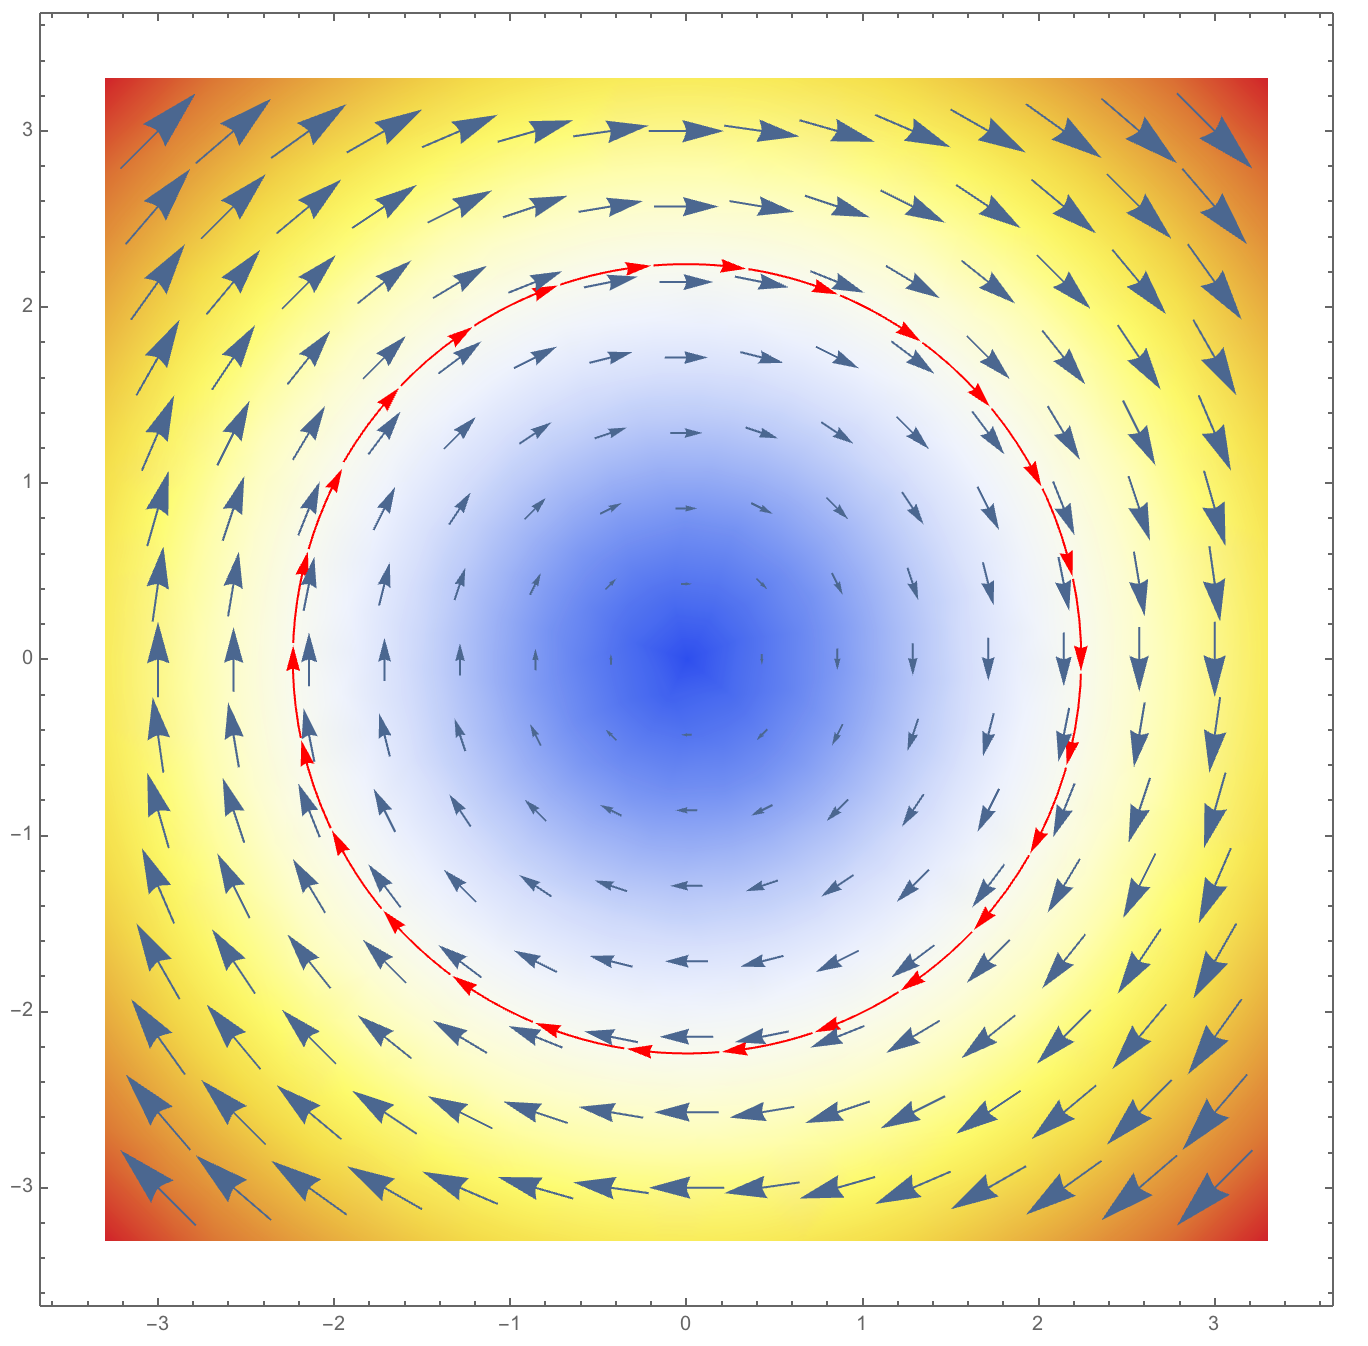
\includegraphics[width=0.5\textwidth]{img/III_CampoCircular.png}
\caption{Campo $D = (y, -x)$ y su correspondiente curva integral $H$.}
\end{wrapfigure}
\end{example}

\begin{example}
Tenemos el campo
\[D = y \dpa{}{x} - x \dpa{}{y}\]

Buscamos las curvas solución $H = cte$ que cumplen $D(H) = 0$.

Operando, tenemos que
\begin{align*}
\dpa{H}{x} &= x \\
\dpa{H}{y} &= y \end{align*}

Integrando en $x$, tendríamos primero que
\[ H(x,y) = \frac{x^2}{2} + C(y) \]
Derivamos con respecto a $y$ y nos queda que
\[ C(y) = \frac{1}{2}y^2\]
y por lo tanto las curvas integrales son
\[ H(x,y) = x^2 + y^2\]


En este caso vamos a querer enderezar el campo, de tal forma que se exprese en función de una coordenada.

La primera coordenada será la integral primera, y lo que tendremos que hacer para enderezar el campo será pasar a polares. Así, las coordenadas serían \begin{align*} F(x,y) &= \sqrt{x^2 + y^2}  \\ G(x,y) &= - \arctan \frac{y}{x} \end{align*} y por lo tanto nos quedaría que \[ D = \dpa{}{G} \]

\end{example}

\begin{example} Nos dan $f(t) = (t,t^2,t^3)$ y nos pien que digamos si es una inmersión, siendo $X = \img f ⊂ ℝ^3$ %y nosequé.

Para ver si es una inmersión, derivamos y $f'(t) = (1, 2t, 3t^2)$. Gracias a ese $1$ $f'$ no se anula, y por el $t$ de $f$ tenemos que es inyectiva. Luego es inyectiva e inmersión en todo punto.

¿Cómo vemos si es una subvariedad? Habría que ver si es compatible con la topología, esto es, si la función inversa es continua en esa topología. La inversa es $\appl{\inv{f}}{X}{ℝ}$ con $\inv{f}(t, t^2, t^3) = t$, perfectamente continua.

La última pregunta es si podemos definir una aplicación $\appl{F}{ℝ^3}{ℝ^2}$ con $X = \inv{F}((0,0))$ tal que $F$ sea una submersión en todos los puntos $x ∈ X$.

$F$ sería\footnote{Se obtiene viendo que si $y-x^2 = 0$ entonces $y = x^2$ y análogamente con la segunda coordenada $z = x^3$. Esto es precisamente lo que decía $f(x) = (x, x^2, x^3)$.} \[ F(x,y,z) = (y-x^2, z-x^3)\]

El jacobiano de esto tendría determinante no nulo. Así, $\inv{F}((a,b))$ es una subvariedad de $ℝ^3$ de dimensión $1$ para todo $(a,b) ∈ ℝ^2$ por el teorema de submersión.

\end{example}

\section{Formas diferenciales en variedades}

Podemos construir el espacio tangente a una variedad $X$ en un punto $x$, de la forma:
\[
T_x^*X = \gen{(dx_1)_x, ... ,  (dx_n)_x}
\]

Si tomamos \[\bigcup T_x^*X =: T^* X \to X\]

Esta construcción se parece a la del fibrado tangente. Esta construcción se denomina \concept{Fibrado cotangente}. Es una familia de espacios lineales parametrizado por los puntos de $X$.

Además, en la unión disjunta se puede definir una topología, con unos abiertos y así acabamos llegando a que es una variedad.

Ahora vamos a definir formas en $X$.

\begin{defn}[1-forma en $X$]
	Una 1-forma en $X$ es una función $\appl{ω}{X}{T^*X}$ tal que \begin{itemize}
		\item Es diferenciable
		\item $π \circ ω = id_x$
	\end{itemize}
\end{defn}

Sea $(U_i, \phi_i)$ una carta local en $X$,  entonces ω tendrá unas coordenadas locales respecto de esa carta, es decir: $ω = \sum a_i(x_1,...,x_n) dx_i$

¿Y cómo cambiamos de coordenadas la 1-forma entre cartas distintas?

Sea $F := \phi_j \circ \phi_j$

\[
\left.\begin{array}{c}
y_1 = y_1(x_1,..,x_n)\\
\vdots\\
y_n = y_n(x_1,...,x_n)\\
\end{array}\right\} F
\]

Para escribir el cambio de coordenadas, $ω_j = \sum b_i dy_i = F^* (ω_i) = F^*\left(\sum a_idx_i\right)$


Se deja como ejercicio para el lector, hacer lo mismo que demostramos para el fibrado tangente, con el fibrado cotangente.


\subsection{p-formas}
Recordamos que las p-formas pertenecen al espacio $Λ^p(T_x^*X)$, ya que son de la forma \[ω = \sum_{i_1<i_2,...,i_p} a_i...a_p dx_1Λ...Λ dx_p\]

Por construcción, tenemos (como teníamos para las 1-formas) que

\[Λ^p(T_x^*X) = \bigcup_{x∈X} Λ^p T_x^*X \to X\]

\begin{defn}[p-forma en $X$]
	Una 1-forma en $X$ es una función $\appl{ω}{X}{\bigcup_{x∈X} Λ^p T_x^*X}$, siendo $π$ su inversa, tal que \begin{itemize}
		\item Es diferenciable
		\item $π \circ ω = id_x$
	\end{itemize}
\end{defn}


Es importante darnos cuenta que los coeficientes de las p-formas ya no son números, sino funciones $C^∞$, ya que el punto $x∈X$ no siempre es el mismo.

\paragraph{¿Y esto no es lo mismo?} Pues aunque lo parezca, y yo también lo crea debe ser que no. La diferencia debe de estar en que antes trabajamos con formas en abiertos de $ℝ^n$ y no en variedades. Lo que nos interesa ahora es ver que las normas de cálculo que teníamos con formas en abiertos, se mantienen en variedades.

\begin{itemize}
\item $ω_pΛω_q'$ es una $p+q$ forma en la misma variedad. Esto se debe a que \[F^*(ωΛω') = F^*(ω) Λ F^*(ω')\]
Esta fórmula sirve para cualquier función diferenciable. Si ponemos en esas $F$ cambios de carta, obtenemos que el producto pinchorial se comporta bien con los cambios de carta.

\item $dω_p$ es una $p+1$-forma que se obtiene igual. Ya vimos que $F^*(dω) = d(F^*ω)$ en abierto de $ℝ^n$. Si lo aplicamos a variedades, $dω_i = d(F^*(ω_j)) = F^*(dω_j)$, siendo $F$ el cambio de carta de en la que definimos $ω_i$ a la que definimos $ω_j$.
\item Hay otras operaciones con formas interensantes (como la derivada de Lie) que no da tiempo a ver y que no utilizaremos durante el curso.
\end{itemize}

Estas propiedades que se mantengan hacen que las formas sean objetos globales de las variedades y no solamente locales.

Nos podríamos plantear cómo se aplican formas a campos. Una 2-forma se aplicará a 2 campos. ¿Existe alguna manera de calcular $dω(D,D')$?

\begin{theorem}[Teorema\IS de Cartan]
Sea $ω$ una 1-forma, y $D,D'$ 2 campos.

\[dω(D,D') = Dω(D') - D'ω(D) - ω([D,D'])\]

\end{theorem}


\begin{proof}
	Sea $ω = f dg$, con lo que $dω = df Λ dg$.

	Por un lado, aplicando lo que ya "sabemos":
	\[dω(D_1,D_2) = df Λ dg(D_1,D_2) \overset{def.}{=} \det\begin{pmatrix}
	df(D_1) & dg(D_1)\\
	df(D_2) & dg(D_2)
	\end{pmatrix}
	\]

	Aplicando Cartan:

	\[
	D_1(ω(D_2)) = D_1(fdg(D_2)) \overset{Leib}{=} D_1(f) D_2(g) + f(D_1D_2g)
	\]

	Es por ese último término por lo que aparece el corchete en la fórmula de Cartan.

	\[D_2(ω(D_1)) = ... = ... = D_2(f)D_1(g) + f(D_1D_2g)	\]

	Y el tercer término que necesitamos para la fórmula,
	\[ω([D_1,D_2]) =fdg([D_1,D_2]) =f[D_1,D_2]g = f(D_1D_2g - D_1D_2g)	\]

	El último paso se deja para el lector.

\end{proof}
Hay que darse cuenta que esta prueba es una prueba local, ya que está hecha con coordenadas.


\begin{example}
	Este ejemplo es del libro de DoCarmo, el 14 del capítulo en el que estamos.

	Dice así:


	Sea $ω = zdx + xdy + y dz$. Nos piden demostrar que no tiene una fórmula integral.

	Queremos una superficie, tal que restringir la 1-forma a la superficie, sea 0, es decir:

	\[ω|_s = 0 \dimplies ω(D) = 0 \; D∈TS \text{( D es un campo tangente)}\]

	Como estamos buscando una superficie, buscamos 2 campos que sean tangentes y que cumplan la condición descrita arriba.

	Show time! Sean $D_1 = x \dpa{}{x} - z\dpa{}{y}$ y $D_2 = y\dpa{}{x} - z\dpa{}{z}$. Estos 2 campos cumplen la condición por construcción.


	Ahora queremos ver si esos 2 campos son coherentes entre sí, es decir, dividen el espacio no se como. Lo que necesitamos ver para que los 2 campos pertenezcan a la distribución (Δ) (que es lo mismo que ser coherente o dividir el espacio nosecomo). Esto es comprobar que $\gen{D_1,D_2} = Δ$. Por el teormea de frobenius, tenemos que 	$ \gen{D_1,D_2} = Δ \dimplies [D_1,D_2]∈Δ$ (tal vez con una única implicación).


	Este sería el camino habitual, pero podemos aplicar la fórmula de Cartan y obtener:

	$d\omega(D_1,D_2) = \underset{D_1\omega(D_2)}{0} - \underset{D_2ω(D_1)}{=0} - ω([D_1,D_2])$


	Si se cumpliera $[D_1,D_2]∈Δ$, tendríamos que $ω([D_1,D_2]) = 0$, con lo que $dω(D_1,D_2) = 0$. Si vemos que $dω(D_1,D_2) ≠ 0$, entonces tendremos que no tiene fórmula integral, porque no tiene ¿distribución?.

	$dω = dz Λ dx + dx Λ dy + dyΛdz$ Si aplicamos estos 3 sumandos, tendremos:

	\[
	dz Λ dx (D_1,D_2) = \det\begin{pmatrix}
	dz(D_1) & dx(D_1) \\ dz(D_2) & dx(D_2)
	\end{pmatrix} = xz
	\]

	Haciendo el cálculo con los otros 2 sumandos de $dω$, obtenemos:

	\[dω(D_1,D_2) = xz + yz * z^2 ≠ 0\]

	Partíamos de $z≠0$ en todo punto. Es por ello que el corchete no puede pertenecer a la distribución generada por los 2 campos. La base de esta no existencia es el sistema de $EDO$ que hay por detrás, que se tienen que dar unas condiciones necesarias para que tenga solución, y en este caso no ha podido ocurrir.

\end{example}
